\ifx\wholebook\relax \else
% ------------------------ 

\documentclass{article}
%------------------- Other types of document example ------------------------
%
%\documentclass[twocolumn]{IEEEtran-new}
%\documentclass[12pt,twoside,draft]{IEEEtran}
%\documentstyle[9pt,twocolumn,technote,twoside]{IEEEtran}
%
%-----------------------------------------------------------------------------
%%
% loading packages
%
\newif\ifpdf
\ifx\pdfoutput\undefined % We're not running pdftex
  \pdffalse
\else
  \pdftrue
\fi
%
%
\ifpdf
  \RequirePackage[pdftex,%
            CJKbookmarks,%
       bookmarksnumbered,%
              colorlinks,%
          linkcolor=blue,%
              hyperindex,%
        plainpages=false,%
       pdfstartview=FitH]{hyperref}
\else
  \RequirePackage[dvipdfm,%
             CJKbookmarks,%
        bookmarksnumbered,%
               colorlinks,%
           linkcolor=blue,%
               hyperindex,%
         plainpages=false,%
        pdfstartview=FitH]{hyperref}
  \AtBeginDvi{\special{pdf:tounicode GBK-EUC-UCS2}} % GBK -> Unicode
\fi
\usepackage{hyperref}

% other packages
%-----------------------------------------------------------------------------
\usepackage{graphicx, color}
\usepackage{CJK}
%
% for programming 
%
\usepackage{verbatim}
\usepackage{listings}


\lstdefinelanguage{Smalltalk}{
  morekeywords={self,super,true,false,nil,thisContext}, % This is overkill
  morestring=[d]',
  morecomment=[s]{"}{"},
  alsoletter={\#:},
  escapechar={!},
  literate=
    {BANG}{!}1
    {UNDERSCORE}{\_}1
    {\\st}{Smalltalk}9 % convenience -- in case \st occurs in code
    % {'}{{\textquotesingle}}1 % replaced by upquote=true in \lstset
    {_}{{$\leftarrow$}}1
    {>>>}{{\sep}}1
    {^}{{$\uparrow$}}1
    {~}{{$\sim$}}1
    {-}{{\sf -\hspace{-0.13em}-}}1  % the goal is to make - the same width as +
    %{+}{\raisebox{0.08ex}{+}}1		% and to raise + off the baseline to match -
    {-->}{{\quad$\longrightarrow$\quad}}3
	, % Don't forget the comma at the end!
  tabsize=2
}[keywords,comments,strings]

\lstloadlanguages{C++, Lisp, Haskell, Python, Smalltalk}

% ======================================================================

\def\BibTeX{{\rm B\kern-.05em{\sc i\kern-.025em b}\kern-.08em
    T\kern-.1667em\lower.7ex\hbox{E}\kern-.125emX}}

\newtheorem{theorem}{Theorem}

%
% mathematics
%
\newcommand{\be}{\begin{equation}}
\newcommand{\ee}{\end{equation}}
\newcommand{\bmat}[1]{\left( \begin{array}{#1} }
\newcommand{\emat}{\end{array} \right) }
\newcommand{\VEC}[1]{\mbox{\boldmath $#1$}}

% numbered equation array
\newcommand{\bea}{\begin{eqnarray}}
\newcommand{\eea}{\end{eqnarray}}

% equation array not numbered
\newcommand{\bean}{\begin{eqnarray*}}
\newcommand{\eean}{\end{eqnarray*}}

\RequirePackage{CJK,CJKnumb,CJKulem,CJKpunct}
% we use CJK as default environment
\AtBeginDocument{\begin{CJK*}{GBK}{song}\CJKtilde\CJKindent\CJKcaption{GB}}
\AtEndDocument{\clearpage\end{CJK*}}

%
% loading packages
%

\RequirePackage{ifpdf}

%
%
\ifpdf
  \RequirePackage[pdftex,%
       bookmarksnumbered,%
              colorlinks,%
          linkcolor=blue,%
              hyperindex,%
        plainpages=false,%
       pdfstartview=FitH]{hyperref}
\else
  \RequirePackage[dvipdfm,%
        bookmarksnumbered,%
               colorlinks,%
           linkcolor=blue,%
               hyperindex,%
         plainpages=false,%
        pdfstartview=FitH]{hyperref}
\fi
\usepackage{hyperref}

% other packages
%--------------------------------------------------------------------------
\usepackage{graphicx, color}
\usepackage{subfig}

\usepackage{amsmath, amsthm, amssymb} % for math
\usepackage{exercise} % for exercise

%
% for programming 
%
\usepackage{verbatim}
\usepackage{listings}
%\usepackage{algorithmic} %old version; we can use algorithmicx instead
\usepackage{algorithm} 
\usepackage[noend]{algpseudocode} %for pseudo code, include algorithmicsx automatically
\usepackage{makeidx} % for index support


\lstdefinelanguage{Smalltalk}{
  morekeywords={self,super,true,false,nil,thisContext}, % This is overkill
  morestring=[d]',
  morecomment=[s]{"}{"},
  alsoletter={\#:},
  escapechar={!},
  literate=
    {BANG}{!}1
    {UNDERSCORE}{\_}1
    {\\st}{Smalltalk}9 % convenience -- in case \st occurs in code
    % {'}{{\textquotesingle}}1 % replaced by upquote=true in \lstset
    {_}{{$\leftarrow$}}1
    {>>>}{{\sep}}1
    {^}{{$\uparrow$}}1
    {~}{{$\sim$}}1
    {-}{{\sf -\hspace{-0.13em}-}}1  % the goal is to make - the same width as +
    %{+}{\raisebox{0.08ex}{+}}1		% and to raise + off the baseline to match -
    {-->}{{\quad$\longrightarrow$\quad}}3
	, % Don't forget the comma at the end!
  tabsize=2
}[keywords,comments,strings]

\lstloadlanguages{C++, Lisp, Haskell, Python, Smalltalk}

% ======================================================================

\def\BibTeX{{\rm B\kern-.05em{\sc i\kern-.025em b}\kern-.08em
    T\kern-.1667em\lower.7ex\hbox{E}\kern-.125emX}}

%
% mathematics
%
\newcommand{\be}{\begin{equation}}
\newcommand{\ee}{\end{equation}}
\newcommand{\bmat}[1]{\left( \begin{array}{#1} }
\newcommand{\emat}{\end{array} \right) }
\newcommand{\VEC}[1]{\mbox{\boldmath $#1$}}

% numbered equation array
\newcommand{\bea}{\begin{eqnarray}}
\newcommand{\eea}{\end{eqnarray}}

% equation array not numbered
\newcommand{\bean}{\begin{eqnarray*}}
\newcommand{\eean}{\end{eqnarray*}}

\newtheorem{theorem}{Theorem}[section]
\newtheorem{lemma}[theorem]{Lemma}
\newtheorem{proposition}[theorem]{Proposition}
\newtheorem{corollary}[theorem]{Corollary}


\setcounter{page}{1}

\begin{document}

\fi
%--------------------------

% ================================================================
%                 COVER PAGE
% ================================================================

\title{Searching}

\author{Larry~LIU~Xinyu
\thanks{{\bfseries Larry LIU Xinyu } \newline
  Email: liuxinyu95@gmail.com \newline}
  }

\markboth{Searching}{AlgoXY}

\maketitle

\ifx\wholebook\relax
\chapter{Searching}
\numberwithin{Exercise}{chapter}
\fi

% ================================================================
%                 Introduction
% ================================================================
\section{Introduction}
\label{introduction} 
Searching is a quite big and important area. Computer turns many hard
searching problem realistic, which is almost impossible for human begins.
A modern industry robot can even search and pick the correct gadget from
the pipeline for assembly; A GPS car navigator can search among the
map, for the best route to a specific place. The modern mobile phone
does not only equipped with such map navigator, but can also search
for internet shopping with the best price.

This chapter just scratch the surface of elementary searching. One
good thing that computer offers is the brute-force scanning for a
certain result in a large sequences. The divide and conquers
search strategy will be briefed with two problems, one is to find
the $k$-th big one among a list of unsorted elements; the other
is the popular binary search among a list of sorted elements.
We'll also introduce the extension of binary search for searching
among multiple-dimension data.

Text matching is also very important in our daily life, two well-known
searching algorithms, Knuth-Morris-Pratt (KMP) and Boyer-Moore algorithm
will be introduced, They set good example for another searching strategy:
information reusing.

Besides sequence search, some elementary methods for searching
solution of some interesting problems will be introduced. They
were mostly well studied in the early phase of AI (artificial
intelligence), including the basic DFS (Depth first search), 
and BFS (Breadth first search).

Finally, Dynamic programming will be briefed for searching
optimal solutions, and we'll also introduce about greedy
algorithm which is applicable for some special cases.

All algorithms will be realized in both imperative and functional
approaches.

% ================================================================
% Sequence search
% ================================================================
\section{Sequence search}

%% \begin{figure}[htbp]
%%  \centering
%%  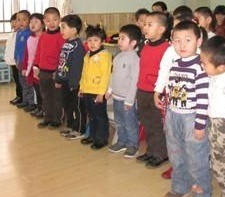
\includegraphics[scale=0.8]{img/kids-inline.eps}
%%  \caption{Instruct kids to stand in a line}
%%  \label{fig:knuth-ssort}
%% \end{figure}

%% \begin{tabular}{ | c c c c c c c c |}
%% \hline
%% {\bf 102} & 100 & 98 & 95 & 96 & 99 & 101 & 97 \\
%% {\bf 100} & 98 & 95 & 96 & 99 & 101 & 97 & {\em 102} \\
%% {\bf 98} & 95 & 96 & 99 & 97 & {\em 100} & 101 & {\em 102} \\
%% {\bf 95} & 96 & 97 & {\em 98} & 99 & {\em 100} & {\em 101} & {\em 102} \\
%% {\em 95} & {\bf 96} & 97 & {\em 98} & {\em 99} & {\em 100} & {\em 101} & {\em 102} \\
%% {\em 95} & {\em 96} & 97 & {\em 98} & {\em 99} & {\em 100} & {\em 101} & {\em 102} \\
%% {\em 95} & {\em 96} & {\em 97} & {\em 98} & {\em 99} & {\em 100} & {\em 101} & {\em 102} \\
%% \hline
%% \end{tabular}

\subsection{Divide and conquer search}

\subsubsection{k-th element problem}

%% \be
%% sort(L) = \left \{
%%   \begin{array}
%%   {r@{\quad:\quad}l}
%%   \Phi & L = \Phi \\
%%   sort(\{ x | x \in L', x \leq l_1 \} \cup \{ l_1 \} \cup sort(\{ x | x \in L', l_1 < x \}) & otherwise \\
%%   \end{array}
%% \right.  
%% \ee

\subsubsection{binary search}

\subsubsection{2 demension bineary search? Dijkstra}

\subsection{Information reuse}

\subsubsection{KMP}

\subsubsection{Boyer-moore}

\section{Solution searching}
\subsection{DFS and BFS}

\subsection{Search the optimal solution}

\subsection{Dynamic programming}

\subsection{Grady algorithm}

\section{Short summary} 
summary

\begin{thebibliography}{99}

\bibitem{TAOCP}
Donald E. Knuth. ``The Art of Computer Programming, Volume 3: Sorting and Searching (2nd Edition)''. Addison-Wesley Professional; 2 edition (May 4, 1998) ISBN-10: 0201896850 ISBN-13: 978-0201896855

\bibitem{CLRS}
Thomas H. Cormen, Charles E. Leiserson, Ronald L. Rivest and Clifford Stein. 
``Introduction to Algorithms, Second Edition''. ISBN:0262032937. The MIT Press. 2001

\end{thebibliography}

\ifx\wholebook\relax\else
\end{document}
\fi

